% chapter 4 section 4

\section{电磁感应}

\subsection{电磁感应}
\label{subsec:4.4.1}

\subsubsection{楞次定律}

\begin{figure}[ht!]
    \centering
    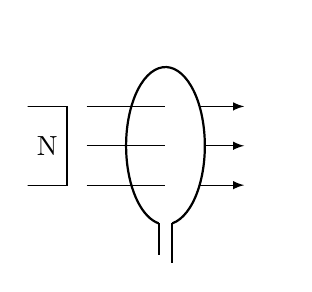
\begin{tikzpicture}[scale=0.5]
        \clip (-3.5,-3) rectangle (3,3);
        \draw (-4,-1) rectangle (-2.5,1);
        \node at (-3,0) {N};
        \foreach \y in {-1,0,1} \draw[-latex] (0,\y) -- (2,\y);
        \filldraw[thick, draw=black, fill=white] (-80:1 and 2) arc (-80:260:1 and 2);
        \draw[thick] (-80:1 and 2) -- ++ (0,-1);
        \draw[thick] (260:1 and 2) -- ++ (0,-0.8);
        \foreach \y in {-1,0,1} \draw (-2,\y) -- (0,\y);
    \end{tikzpicture}
    \caption{楞次定律}
\end{figure}
实验表明磁场的变化会激发出相应的电的效果,即电磁感应现象,日文为電磁誘導。其中称激发出来的电流为感应电流(誘導電流),称与之对应的起电力为感应电势(誘導起電力)。描述其感应电流方向的定律为楞次定律,日文为レンツの法則。
\begin{itembox}[l]{楞次定律}
    \centering
    变化的磁场会产生妨碍该变化的感应电流/电势(增反减同)
\end{itembox}

\subsubsection{法拉第电磁感应定律}

日文为ファラデーの電磁誘導の法則,其定量地描述了磁生电的效果。为此我们需要率先明确磁通量的概念。

磁通量,日文为磁束,是描述给定面上磁场大小的量,一般用字母$\Phi$表示。应注意只有与给定面垂直的部分才会被计为磁通量。
\begin{equation*}
    \Phi=B\cdot S
\end{equation*}

至此,磁生电的现象则可由磁通量随时间的变化描述,即法拉第电磁感应定律。
\begin{equation*}
    V=-\frac{\Delta\Phi}{\Delta t}
\end{equation*}

\subsubsection{运动导体的感应电势}

\paragraph{一般模型}实际题目中常常很难直接使用法拉第电磁感应定律,而是更多使用其在特定模型下的形式。题目中常见的模型如下,空间中布满匀强磁场,平行金属导轨上有一根可移动的金属棒,让金属棒以一定速度运动,探究此时的感应电势。
\begin{figure}[ht!]
    \centering
    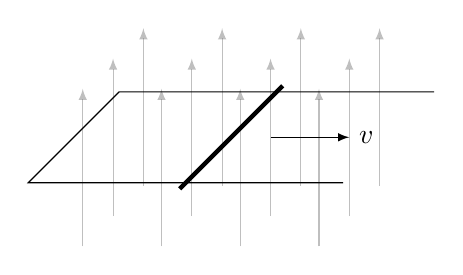
\begin{tikzpicture}
        \foreach \x in {0.5,1.5,2.5,3.5} \foreach \z in {0.5,1.5,2.5}
            \draw[-latex,color=gray,opacity=0.5] (\x,-1,\z) -- (\x,1,\z);
        \draw (4,0,0) -- (0,0,0) -- (0,0,3) -- (4,0,3);
        \draw[ultra thick] (2,0,-0.2) -- (2,0,3.2);
        \draw[-latex] (2.5,0,1.5) -- (3.5,0,1.5) node[right] {$v$};
    \end{tikzpicture}
    \caption{电磁感应水平模型}
\end{figure}
根据法拉第电磁感应定律可得感应电势大小为
\begin{equation*}
    |V|=\frac{\Delta\Phi}{\Delta t}=\frac{BS}{t}=\frac{B\Delta xl}{\Delta t}=Bvl
\end{equation*}
其方向可由楞次定律或者右手定则判断。
\begin{itemize}
    \item 磁场穿过手心
    \item 拇指与运动方向同向
    \item 四指为电流方向
\end{itemize}

\paragraph{斜面模型}时而题目中会出现斜向的平行导轨。
\begin{figure}[ht!]
    \centering
    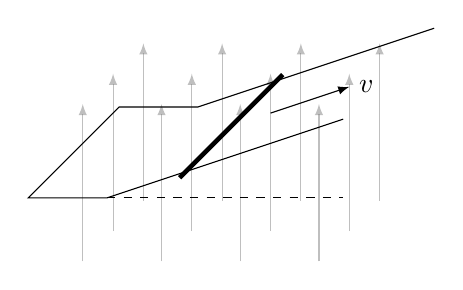
\begin{tikzpicture}
        \foreach \x in {0.5,1.5,2.5,3.5} \foreach \z in {0.5,1.5,2.5}
            \draw[-latex,color=gray,opacity=0.5] (\x,-1,\z) -- (\x,1,\z);
        \draw (4,1,0) -- (1,0,0) -- (0,0,0) -- (0,0,3) -- (1,0,3) -- (4,1,3);
        \draw[dashed] (1,0,3) -- (4,0,3);
        \drawangle{(4,0,3)}{(1,0,3)}{(4,1,3)};
        \draw[ultra thick] (2,1/3,-0.2) -- (2,1/3,3.2);
        \draw[-latex] (2.5,0.5,1.5) -- (3.5,5/6,1.5) node[right] {$v$};
    \end{tikzpicture}
    \caption{电磁感应斜面模型}
\end{figure}
此时实际与金属棒运动方向垂直的磁通量密度为$B\cos\theta$,根据磁通量的定义可得
\begin{equation*}
    V=Bvl\cos\theta
\end{equation*}

\paragraph{圆环模型}此外题目中偶尔也会出现稍复杂一些的圆环模型。
\begin{figure}[ht!]
    \centering
    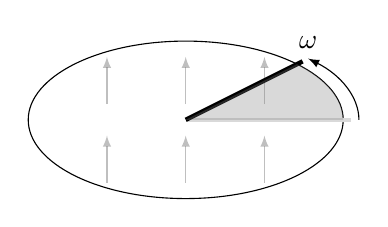
\begin{tikzpicture}
        \foreach \x in {-1,0,1} \foreach \y in {-0.5,0.5}
            \draw[-latex,color=gray,opacity=0.5] (\x,{\y-0.3}) -- (\x,{\y+0.3});
        \draw (0,0) circle (2 and 1);
        \draw[ultra thick, color=gray!30] (0,0) --(2.1,0);
        \draw[ultra thick] (0,0) -- (45:2.1 and 1.05);
        \draw[-latex] (2.2,0) arc (0:45:2.2 and 1.1) node[above] {$\omega$};
        \fill[color=gray,opacity=0.3] (0,0) -- (2,0) arc (0:45:2 and 1) --cycle;
    \end{tikzpicture}
    \caption{电磁感应圆环模型}
\end{figure}
根据扇形公式可知,在$\Delta t$的时间内金属棒会扫过$\Delta S=\frac12\omega\Delta tl^2$的面积,结合法拉第电磁感应定律可得
\begin{equation*}
    V=\frac12\omega Bl^2
\end{equation*}

\subsubsection{自感与互感}

\paragraph{自感现象} 思考一个接入了线圈的闭合直流电路,当电源闭合时电路内电流增大。根据线圈磁场的知识可知,线圈内会产生一个逐渐增大的磁场,因此相应地会激发出电磁感应现象,生成出一个阻碍该变化的感应电流减缓电路内的电流增长。相对的,当电源断开时电路内电流减少,线圈内会产生一个逐渐减小的磁场,随之而来的感应电流也会阻碍这个减少的变化。我们称这个现象为\underline{自感},日文为自己誘導。

根据法拉第电磁感应定律即可求出实现线圈阻碍效果的感应电势的大小。
\begin{equation*}
    V=-N\frac{\Delta\Phi}{\Delta t}
    =-N\frac{\mu n\Delta IS}{\Delta t}
    =-\mu n^2lS\frac{\Delta I}{\Delta t}
\end{equation*}
一般记为$V=-L\frac{\Delta I}{\Delta t}$,其中的$L$为自感系数,日文为自己インダクタンス。此外,不难想见自感线圈在电路中对电流起到的是阻碍效果,载流子为了克服该阻碍则需额外做功,这些能量便成为了线圈所能够累积的能量,其大小为
\begin{equation*}
    U=\frac12LI^2
\end{equation*}
在此读者可简单思考其与电容器储能的异同。

\paragraph{互感现象} 思考两个包含线圈的电路,其中一个连接直流电源,另一个连接电阻,且两个线圈连续放置。可以想见当连接电源的线圈激发出变化磁场时,一定会导致另一个线圈内的磁场发生相应变化,从而使其发生电磁感应现象。我们称这个现象为\underline{互感},日文为相互誘導。其感应电势大小为$V=-M\frac{\Delta I}{\Delta t}$,其中的$M$为互感系数,日文为相互インダクタンス。

生活中的变压器便是互感现象的应用实例。假设由铁芯串在一起的两组线圈的匝数分别为$N_1$和$N_2$,那么根据法拉第电磁感应定律可知
\begin{equation*}
    \begin{cases}
        V_1=-N_1\frac{\Delta\Phi}{\Delta t}\\
        V_2=-N_2\frac{\Delta\Phi}{\Delta t}\\
    \end{cases}
\end{equation*}
即$V_1:V_2=N_1:N_2$。此外由于传输过程中功率是共通的,所以两组电路中的电流比为匝数反比。

\subsection{交流电}
\label{subsec:4.4.2}

\subsubsection{产生机制}

一般称周期性改变大小与方向的电流/电压为交流电。若将旋转中的线圈置入恒定的磁场中,则可得到最简单的交流发生装置。
\begin{figure}[ht!]
    \centering
    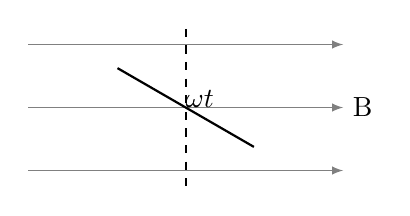
\begin{tikzpicture}
        \foreach \y in {-0.8, 0, 0.8}
            \draw[-latex, color=gray] (-2,\y) -- (2,\y);
        \node[right] at (2,0) {B};
        \draw[thick, dashed] (90:1) -- (-90:1);
        \draw[thick] (150:1) -- (-30:1);
        \drawangle[$\omega t$]{(90:1)}{(0,0)}{(150:1)};
    \end{tikzpicture}
    \caption{交流电的产生}
\end{figure}
可见在任一时刻,实际穿过线圈的磁通量为$\Phi_0\cos\omega t$。根据法拉第电磁感应定律可知,变化的磁通量产生的电压为
\begin{equation*}
    V=-\frac{d\Phi}{dt}=\Phi_0\omega\sin\omega t=V_0\sin\omega t
\end{equation*}
因此,在任一时刻会为连接着负载为$R$的电路提供
\begin{equation*}
    P=IV
    =\frac{V_0}{R}\sin\omega t\times V_0\sin\omega t
    =I_0V_0\sin^2\omega t
\end{equation*}
大小的瞬时电功率。纵观整个周期,
\begin{figure}[ht!]
    \centering
    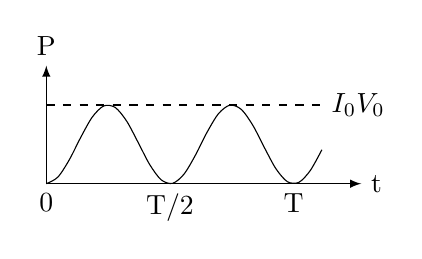
\begin{tikzpicture}
        \draw[-latex] (0,0) -- (4,0) node[right] {t};
        \draw[-latex] (0,0) -- (0,1.5) node[above] {P};
        \draw[solid, domain=0:3.5] plot[smooth] (\x, {sin(2*\x r)^2});
        \node[below] at (0,0) {0};
        \node[below] at ({pi/2},0) {T/2};
        \node[below] at ({pi},0) {T};
        \draw[dashed] (0,1) -- (3.5,1) node[right] {$I_0V_0$};
    \end{tikzpicture}
    \caption{交流电的电功率}
\end{figure}
可知其平均电功率为
\begin{equation*}
    \bar{P}=\frac{I_0V_0}{2}
\end{equation*}
即然周期内的总功率一定,换一种视角则可将交流电视为某个电压/电流恒定的电源,即交流电的实效值为
\begin{gather*}
    I_eV_e=\frac12I_0V_0\\
    \frac{V_e}{R}V_e=\frac12\frac{V_0}{R}V_0\\
    V_e=\frac{V_0}{\sqrt2}
\end{gather*}

\subsubsection{交流电路}

与直流电路不同,交流电路中电源电压的大小与方向呈周期性变化,而且在一些电子元件的作用下电流时而会出现与电压变化不同步的现象。即电压与电流的位相会不一致。

\paragraph{电容器} 对于只含电容器的交流电路,倘若电压为$V=V_0\sin\omega t$,则电路中的电流为$I=\omega CV_0\cos\omega t$。
\begin{figure}[ht!]
    \centering
    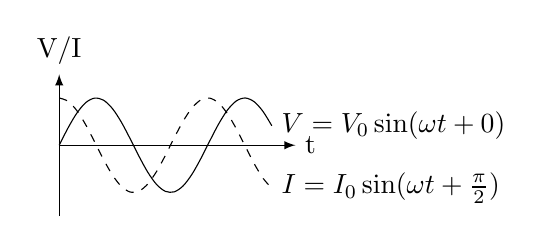
\begin{tikzpicture}[scale=0.6]
        \draw[-latex] (0,0) -- (5,0) node[right] {t};
        \draw[-latex] (0,-1.5) -- (0,1.5) node[above] {V/I};
        \draw[solid, domain=0:4.5] plot[smooth] (\x, {sin(2*\x r)}) node[right] {$V=V_0\sin(\omega t+0)$};
        \draw[dashed, domain=0:4.5] plot[smooth] (\x, {cos(2*\x r)}) node[right] {$I=I_0\sin(\omega t+\frac\pi2)$};
    \end{tikzpicture}
    \caption{交流电中的电容器}
\end{figure}
即电流的变化比电压快$\frac\pi2$。由此不难想象,是因为电容器自身存在着某种阻碍效果才使得电流和电压的位相出现了不一致,在此将这个阻碍效果称为\underline{容抗},日文为容量リアクタンス。
\begin{equation*}
    X_C=\frac{V_e}{I_e}=\frac{1}{\omega C}
\end{equation*}
根据$\omega=2\pi f$可知,交流电频率越低,容抗越大。其极限情况便是频率为0的直流电,电容器会完全阻断电路。此外,在整个周期中电容器的平均功率为0。

\paragraph{线圈} 对于只含线圈的交流电路,倘若电压为$V=V_0\sin\omega t$,则电路中的电流为$I=-\frac{V_0}{\omega L}\cos\omega t$。
\begin{figure}[ht!]
    \centering
    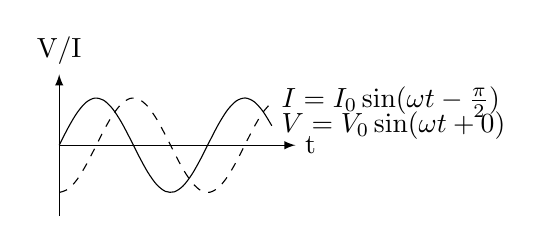
\begin{tikzpicture}[scale=0.6]
        \draw[-latex] (0,0) -- (5,0) node[right] {t};
        \draw[-latex] (0,-1.5) -- (0,1.5) node[above] {V/I};
        \draw[solid, domain=0:4.5] plot[smooth] (\x, {sin(2*\x r)}) node[right] {$V=V_0\sin(\omega t+0)$};
        \draw[dashed, domain=0:4.5] plot[smooth] (\x, {-cos(2*\x r)}) node[right] {$I=I_0\sin(\omega t-\frac\pi2)$};
    \end{tikzpicture}
    \caption{交流电中的电容器}
\end{figure}
即电流的变化比电压慢$\frac\pi2$。因而,线圈自身也存在阻碍效果,即\underline{感抗},日文为誘導リアクタンス。
\begin{equation*}
    X_L=\frac{V_e}{I_e}=\omega L
\end{equation*}
根据$\omega=2\pi f$可知,交流电频率越低,感抗越小。其极限情况便是频率为0的直流电,线圈与导线无异。此外,在整个周期中线圈的平均功率为0。

\subsubsection{RLC震荡电路}

\textbackslash\textbackslash TODO
